\documentclass[12pt,a4paper]{article}
\usepackage{amsmath}
\usepackage{amsthm}
\usepackage[main=hungarian,english]{babel}
\usepackage{float}
\usepackage{graphicx}
\graphicspath{{./images/}}
\usepackage{wrapfig}
\usepackage{tabularx}


\usepackage{minted}


\title{\textbf{Programozási technológia \\ \large  I. Beadandó feladat}}
\author{Boda Bálint \\ KDHPNI}
\date{2022. 10. 10.}

\theoremstyle{definition}

\newenvironment{exercise}
{\begin{definition}[exercise]}
	{\end{definition}}

\newenvironment{solution}
{\begin{definition}[solution]}
	{\end{definition}}

\newtheorem*{remark}{Megjegyzés}
\newtheorem*{exercise*}{Feladat}
\newtheorem*{solution*}{Megoldás}

\begin{document}
	\maketitle
	\section{Feladat}
	Töltsön fel egy gyűjteményt különféle szabályos (kör, szabályos háromszög, négyzet, szabályos hatszög) síkidomokkal! \textbf{Adja meg melyik síkidom befoglaló téglalapja a legnagyobb területű!} Egy síkidom befoglaló téglalapja lefedi a síkidomot, oldalai párhuzamosak a tengelyekkel. Minden síkidom reprezentálható a középpontjával és az oldalhosszal, illetve a sugárral, ha feltesszük, hogy a sokszögek esetében az egyik oldal párhuzamos a koordináta rendszer vízszintes tengelyével, és a többi csúcs ezen oldalra fektetett egyenes felett helyezkedik el. A síkidomokat szövegfájlból töltse be! A fájl első sorában szerepeljen a síkidomok száma, majd az egyes síkidomok. Az első jel azonosítja a síkidom fajtáját, amit követnek a középpont koordinátái és a szükséges hosszúság. A feladatokban a beolvasáson kívül a síkidomokat egységesen kezelje, ennek érdekében a síkidomokat leíró osztályokat egy közös ősosztályból származtassa!
	\newpage
	\section{Terv}
	\subsection{Típusok}
	Minden osztályban felüldefiniáljuk \mintinline{java}|java.lang.Object| osztályból megörökölt \mintinline{java}|toString()| metódust.
	\subsubsection{Point}
	A síkidomok középpontjának reprezentálásához bevezetjük a két dimenziós pontokat ábrázoló \mintinline{Java}|Point| osztályt, mely két adattaggal (\mintinline{Java}|double x,y|) rendelkezik. Az osztály egyetlen egy az adattagokat beállító konstrukorral rendelkezik. 
	
	\subsubsection{Shape}
	A különböző síkidomokat a \mintinline{Java}|Shape| absztrakt ősosztályból származtatjuk, mely egy adattagot tartalmaz, a középpontot (\mintinline{Java}|Point center|). Annak érdekében, hogy egységesen tudjuk kezelni a síkidom objektumokat itt kerül deklarálásra a befoglaló téglalap területét kiszámoló \mintinline{Java}| boundingArea()| metódus.
	\noindent
	A feladatban szereplő síkidomokat két csoportra osztatjuk:
	\begin{enumerate}
		\item Szabályos sokszögek (pl. négyzet, szabályos háromszög és hatszög)
		\item Nem sokszögek (pl. kör)
	\end{enumerate}

	\subsubsection{RegularAbstractPolygon}
	A szabályos sokszögeket egy köztes absztrakt osztályból a \mintinline{java}|Shape| osztályból származtatott \mintinline{java}|AbstractRegularPolygon| osztályból származtatjuk. Ebben az osztályban kerül bevezetésre az oldalhossz mező.
	
	\subsubsection{Konkrét síkidomok}
	A kör osztályt a \mintinline{java}|Shape| osztályból származtatjuk, így fel tudunk venni egy sugár nevű mezőt anélkül, hogy lenne egy felesleges megörökölt oldalhossz mezőnk (ezért nem vettük fel az oldalhossz mezőt a \mintinline{java}|Shape| osztályban).
	\\[8pt]
	A többi (\mintinline{java}|EquilateralTriangle|, \mintinline{java}|Square|, \mintinline{java}|RegularHexagon|) síkidomot az \mintinline{java}|RegularAbstractPolygon| osztályból származtatjuk.
	\\[8pt]
	Minden nem absztrakt síkidom osztályban (\mintinline{java}|EquilateralTriangle|, \mintinline{java}|Square|, \mintinline{java}|RegularHexagon|, \mintinline{java}|Circle|) felüldefiniáljuk a  \mintinline{java}|boundingArea()| metódust.
	\\[18pt]
	A bementi fájlokban a síkidomokat a következő karakterek azonosítják:
	\begin{center}
	\begin{tabular}{|c|c|}
		\hline
		Karakter & Síkidom \\
		\hline
		c & kör \\
		\hline
		s & négyzet \\
		\hline
		t & szabályos háromszög \\
		\hline
		h & szabályos hatszög \\
		\hline
	\end{tabular}
	\end{center}
	\subsubsection{Kivételek}
	Bevezetjük a \mintinline{java}|InvalidFormatException| és a \mintinline{java}|UnknownShapeTypeException| kivételeket, melyek akkor lépnek fel, ha nem megfelelő a bemeneti fájlban szereplő adatok formátuma, valamint, ha olyan karaktert tartalmaz a fájl, melyhez nincs rendelve semmilyen síkidom. 

	\subsubsection{Shapes}
	A \mintinline{java}|Shapes| osztályban, egy síkidomokat tároló adatszerkezetet veszünk fel és itt definiáljuk a beolvasást végző \mintinline{java}|readShapes()| függvényt. A feladat tényleges kérdését a \mintinline{java}|getShapeWithBABR()| metódus válaszolja meg, mely kiválasztja az adott Shapos objektum legnagyobb területű befoglaló téglalappal rendelkező  síkidomot.
	
	\subsection{Osztálydiagramm}
	\begin{figure}[H]
		\centering
		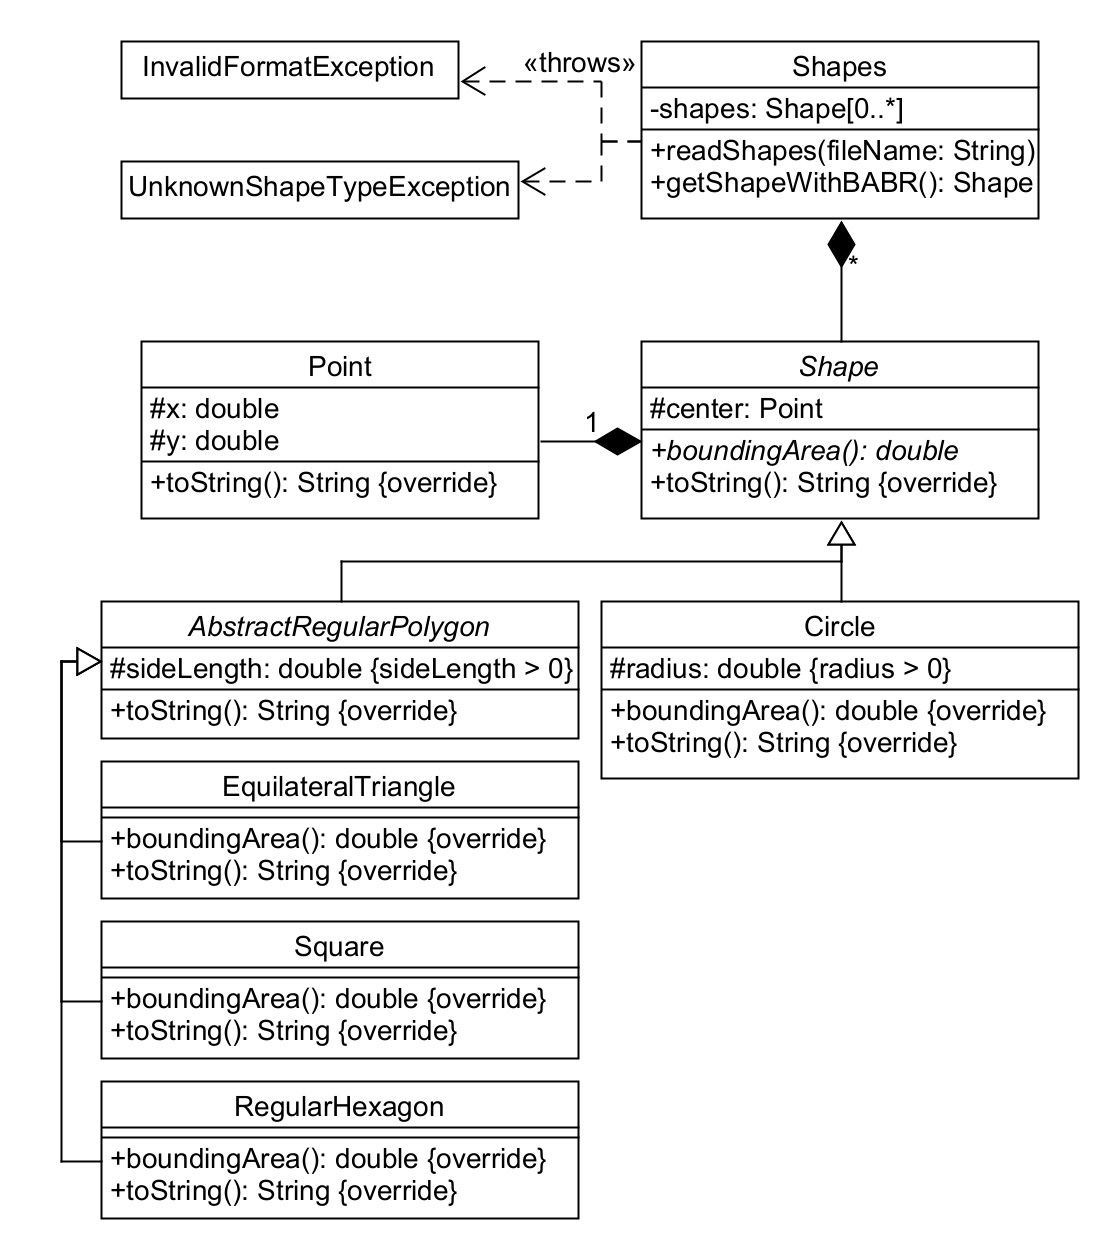
\includegraphics[scale=0.35]{classdiagram.png}
	\end{figure}
	\subsection{Implementálás}
	A terv implementálását a \mintinline{java}|Point| osztállyal érdemes kezdeni (mivel ez más osztálytól nem függ). Ezt követően az általánosabb osztályoktól a specifikusabb osztályok felé érdemes haladni.
	\\[4pt] 
	\textbf{Használt Java verzió: 17.0.4.1}
	\section{Tesztelés}
	\subsection{Fehérdobozos tesztesetek}
	\begin{tabularx}{\textwidth}{|X|l|l|}
		\hline
		Leírás & Bemenet & Elvárt eredmény \\
		\hline
		\raggedright Nem létező fájl & shapesN.txt & FileNotFoundException \\
		\hline
		\raggedright Üres fájl & shapes00.txt  & InvalidFormatException \\
		\hline
		\raggedright Rossz formátumú fájl \#1 & shapesW1.txt & InvalidFormatException \\
		\hline
		\raggedright Rossz formátumú fájl \#2 & shapesW2.txt & InvalidFormatException \\
		\hline
		\raggedright Ismeretlen síkidomtípust tartalmazó fájl & shapesU.txt & UnknownShapeTypeException \\
		\hline
		\raggedright Illegális argumentumú konstruktor hívást eredményező fájltartalom & shapesI.txt & IllegalArgumentException \\
		\hline
	\end{tabularx}

	\subsection{Feketedobozos tesztesetek}
		\begin{tabularx}{\textwidth}{| X | l | X |}
		\hline
		Leírás & Bemenet & Elvárt eredmény \\
		\hline
		\raggedright 0 síkidom & shapes0.txt & null \\
		\hline
		\raggedright Egy síkidom  & shapes1.txt & Circle(radius: 5.0, center: (2.0, 5.0)) \\
		\hline
		\raggedright Több síkidom & shapes2.txt & Circle(radius: 6.0, center: (2.0, 5.0)) \\
		\hline
		\raggedright Extra adatok valahány sorban & shapesE.txt & Circle(radius: 6.0, center: (2.0, 5.0)) \\
		\hline
		\raggedright Több (kb. azonos oldalhosszú) síkidom  & shapes3.txt & RegularHexagon(sideLength: 5.0, center: (0.0, 0.0)) \\
		\hline
		\raggedright Azonos méretű \newline befoglaló téglalap & shapes4.txt & Square(sideLength: 10.0, center: (0.0, 0.0)) \\
		\hline 
	\end{tabularx}
	\subsection{Automatikus tesztelés}
	Az utóbbi tesztesetek a \textbf{BBRTest.java} fájlban szereplő JUnit 5-öt használó tesztkörnyezet részét képezik.
\end{document}